\documentclass[11pt]{article}

\usepackage[a4paper,margin=2cm]{geometry}
\usepackage[utf8]{inputenc}
\usepackage[T1]{fontenc}
\usepackage{longtable}
\usepackage{booktabs}
\usepackage{siunitx}
\usepackage{graphicx}

\sisetup{
    scientific-notation = true,
    round-mode = figures,
    round-precision = 3,
    exponent-product = \times,
}

\title{FFJM2 vs.\ BFGS on the MGH Problems}
\author{}
\date{}

\begin{document}
\maketitle

\noindent
FFJM2 minimizes $\frac{1}{2}\|F(x)\|^2$ with a local quartic model of the
residuals instead of a line search. At iteration $k$, the step $d$ solves
\[
    M_k(d) = \mu\|d\|^2 + \frac{1}{2}\sum_i q_i(d)^2, \qquad
    q_i(d) = r_i + J_i d + \frac{1}{2} d^\top H_i d,
\]
where $r_i$ and $J_i$ are the $i$-th residual and its Jacobian row at
$x_k$, $H_i$ is the current approximation to the Hessian of that residual
component, and $\mu\|d\|^2$ is a Levenberg-Marquardt penalty that damps the
step in place of a line search. The candidate $x_k+d$ is accepted or
rejected based on the ratio between the actual and the predicted reduction
in $f$.

The first iteration starts at
$\mu = 1$. Each accepted step divides $\mu$ by a fixed factor $\mu_{grow} = 10$, with a floor
$\mu_{\min} = 1^{-8}$, so $\mu$ keeps shrinking. Each rejected step instead
multiplies $\mu$ by that same factor $\mu_{grow} = 10$ and re-solves the subproblem at the
same point, until a step is accepted or $\mu$ reaches a ceiling
$\mu_{\max} = 1^{12}$. Unlike a scheme that resets $\mu$ at the start of every
iteration, this value always carries over from the previous one. This
carryover performed better in practice than restarting $\mu$ from scratch
each time.

Every run reported below stops under one of three point-wise criteria,
evaluated with the same default tolerances for \texttt{ffjm2} and for
Optim.jl's \texttt{BFGS} \cite{Mogensen2018} (kept equal so the comparison
is fair):
\begin{itemize}
    \item \textbf{Gradient}: the gradient norm reaches $\|\nabla f\| \le 10^{-8}$. This is a genuine first-order stationary point.
    \item \textbf{Step}: the last step has (numerically) zero length. The solver stalls and stops making progress.
    \item \textbf{Function}: the objective value does not change between two consecutive iterations. The iterate is stuck on a plateau.
    \item \textbf{Stalled}: FFJM2's regularization parameter exceeded its
    ceiling (or its number of consecutive rejections exceeded its cap)
    before any step was accepted. Unlike the first three, this is
    \emph{not} a converged outcome.
\end{itemize}
A run that exhausts the iteration budget without meeting any of the first
three would be reported separately as \emph{not converged}. This case
does not appear in Tables~\ref{tab:hessian-models} and
\ref{tab:psb-vs-sr1} below, but it does in
Table~\ref{tab:psb-vs-bfgs}: FFJM2 (PSB) now stops under the
\textbf{Stalled} criterion on MGH10, MGH16, and MGH31 (the same three
problems that previously stopped under Step/Function --- see the
discussion after that table).

Table~\ref{tab:hessian-models} compares the six ffjm2 Hessian-update
models, each run independently on the 34 MGH least-squares problems
\cite{MoreGarbowHillstrom1981}. Its ``Converged (gradient)'' column counts
how many of the 34 problems stopped under the gradient criterion; the
remaining columns are mean~$\pm$~standard deviation over the 34 problems.
The models are plain BFGS and SR1, the Dennis-Wolkowicz update
\cite{DennisWolkowicz1993} (DW) and its interval-scaled variant
\cite{LuksanSpedicato2000} (IS+DW), interval-scaled BFGS
\cite{LuksanSpedicato2000} (IS+BFGS), and Powell-Symmetric-Broyden
\cite{Powell1970} (PSB).

\begin{table}[htbp]
\centering
\caption{Comparison of the ffjm2 Hessian-update models on the 34 MGH problems.}
\label{tab:hessian-models}
\begin{tabular}{l r r r r r}
\toprule
Model & Converged (gradient) & Iterations & Func.\ evals & Grad.\ evals & Time (s) \\
\midrule
BFGS & 29/34 & $56.88 \pm 188.25$ & $99.97 \pm 351.85$ & $57.88 \pm 188.25$ & $2.071 \pm 6.121$ \\
SR1 & 32/34 & $23.12 \pm 54.84$ & $44.32 \pm 112.92$ & $24.12 \pm 54.84$ & $0.934 \pm 2.992$ \\
IS+BFGS & 29/34 & $44.00 \pm 170.39$ & $88.15 \pm 343.34$ & $45.00 \pm 170.39$ & $1.590 \pm 5.763$ \\
DW & 29/34 & $56.12 \pm 181.91$ & $103.24 \pm 351.45$ & $57.12 \pm 181.91$ & $1.865 \pm 5.942$ \\
IS+DW & 29/34 & $49.41 \pm 173.04$ & $93.74 \pm 344.17$ & $50.41 \pm 173.04$ & $1.768 \pm 5.923$ \\
PSB & 31/34 & $15.68 \pm 22.53$ & $31.38 \pm 53.44$ & $16.68 \pm 22.53$ & $0.424 \pm 0.919$ \\
\bottomrule
\end{tabular}
\end{table}

\noindent
PSB and SR1 are the two best models: together they solve the most problems
under the gradient criterion, and PSB in particular does so with by far the
fewest iterations, evaluations, and execution time on average
(Table~\ref{tab:hessian-models}). SR1 nonetheless certifies gradient
convergence on one more problem than PSB (32/34 against 31/34). To see
exactly where they disagree, Table~\ref{tab:psb-vs-sr1} isolates the three
problems on which at least one of the two methods does not stop under the
gradient criterion.

\begin{longtable}{l l S[table-format=1.3e2] S[table-format=1.3e2] r r l}
\caption{FFJM2 (PSB) vs.\ FFJM2 (SR1): per-problem comparison on the MGH problems.}
\label{tab:psb-vs-sr1} \\
\toprule
Problem & Method & {$f$} & {$\|\nabla f\|$} & {Func.\ evals} & {Grad.\ evals} & Criterion \\
\midrule
\endfirsthead
\caption[]{(continued)} \\
\toprule
Problem & Method & {$f$} & {$\|\nabla f\|$} & {Func.\ evals} & {Grad.\ evals} & Criterion \\
\midrule
\endhead
\midrule
\multicolumn{7}{r}{\textit{continued on next page}} \\
\endfoot
\bottomrule
\endlastfoot
MGH10 & FFJM2 (PSB) & 4.397293e+01 & 5.754922e-05 & 299 & 127 & step \\
MGH10 & FFJM2 (SR1) & 4.397293e+01 & 5.500886e-02 & 297 & 125 & step \\
\midrule
MGH16 & FFJM2 (PSB) & 4.291110e+04 & 9.258506e-05 & 98 & 36 & function \\
MGH16 & FFJM2 (SR1) & 4.291110e+04 & 6.255963e-05 & 44 & 9 & function \\
\midrule
MGH31 & FFJM2 (PSB) & 1.528639e+00 & 2.527165e-08 & 62 & 21 & function \\
MGH31 & FFJM2 (SR1) & 1.528639e+00 & 4.387102e-09 & 44 & 29 & gradient \\
\end{longtable}

\noindent
On MGH10 and MGH16, neither model reaches the gradient criterion: both
stall under the step and function criteria, respectively, at essentially
the same objective value, although FFJM2 with PSB reaches a smaller
gradient norm on MGH10. MGH31 is the one case that favors SR1 over PSB.
SR1 certifies a small gradient norm ($\|\nabla f\| \approx 4.4\times
10^{-9}$), while PSB stops one iteration earlier under the function
criterion, even though both reach practically the same objective value
($f \approx 1.5286$) and gradient norm. For this reason, PSB is the best
choice between the two approaches when weighing cost against benefit.

FFJM2 (PSB) uses persistent decaying $\mu$, a full Hessian reset on a bad
ratio, and $-\nabla f$+Armijo at $k=0$ and as a safeguard. The following
table compares it against BFGS with backtracking line search on the 34
MGH least-squares problems.

\begin{longtable}{l l S[table-format=1.3e2] S[table-format=1.3e2] r r l}
\caption{FFJM2 (PSB) vs.\ BFGS (backtracking): per-problem comparison on the MGH problems.}
\label{tab:psb-vs-bfgs} \\
\toprule
Problem & Method & {$f$} & {$\|\nabla f\|$} & {Func.\ evals} & {Grad.\ evals} & Criterion \\
\midrule
\endfirsthead
\caption[]{(continued)} \\
\toprule
Problem & Method & {$f$} & {$\|\nabla f\|$} & {Func.\ evals} & {Grad.\ evals} & Criterion \\
\midrule
\endhead
\midrule
\multicolumn{7}{r}{\textit{continued on next page}} \\
\endfoot
\bottomrule
\endlastfoot
MGH01 & FFJM2 (PSB) & 2.415715e-22 & 9.822188e-12 & 12 & 8 & gradient \\
MGH01 & BFGS (backtracking) & 1.981121e-22 & 3.687403e-10 & 53 & 40 & gradient \\
\midrule
MGH02 & FFJM2 (PSB) & 5.096567e-18 & 3.844849e-09 & 10 & 7 & gradient \\
MGH02 & BFGS (backtracking) & 1.106930e-26 & 2.198151e-12 & 15 & 11 & gradient \\
\midrule
MGH03 & FFJM2 (PSB) & 1.576836e-11 & 2.568219e-09 & 31 & 20 & gradient \\
MGH03 & BFGS (backtracking) & 5.053640e-30 & 2.830752e-10 & 233 & 174 & gradient \\
\midrule
MGH04 & FFJM2 (PSB) & 3.811648e-17 & 8.733972e-09 & 10 & 8 & gradient \\
MGH04 & BFGS (backtracking) & 9.860761e-32 & 4.440892e-10 & 40 & 14 & gradient \\
\midrule
MGH05 & FFJM2 (PSB) & 1.307511e-16 & 6.948485e-09 & 10 & 8 & gradient \\
MGH05 & BFGS (backtracking) & 2.500895e-22 & 1.079551e-10 & 22 & 19 & gradient \\
\midrule
MGH06 & FFJM2 (PSB) & 1.010000e+03 & 1.161571e-28 & 11 & 2 & gradient \\
MGH06 & BFGS (backtracking) & 1.010000e+03 & 1.161571e-28 & 10 & 2 & gradient \\
\midrule
MGH07 & FFJM2 (PSB) & 1.492293e-17 & 6.034835e-09 & 17 & 10 & gradient \\
MGH07 & BFGS (backtracking) & 5.236320e-19 & 5.028697e-09 & 41 & 30 & gradient \\
\midrule
MGH08 & FFJM2 (PSB) & 4.107439e-03 & 4.903415e-10 & 12 & 9 & gradient \\
MGH08 & BFGS (backtracking) & 4.107439e-03 & 7.394161e-10 & 34 & 28 & gradient \\
\midrule
MGH09 & FFJM2 (PSB) & 5.639664e-09 & 7.549518e-11 & 9 & 7 & gradient \\
MGH09 & BFGS (backtracking) & 5.639664e-09 & 1.552131e-09 & 6 & 5 & gradient \\
\midrule
MGH10 & FFJM2 (PSB) & 4.397293e+01 & 1.204293e-05 & 276 & 122 & stalled \\
MGH10 & BFGS (backtracking) & 4.397293e+01 & 2.281500e+00 & 552 & 386 & step \\
\midrule
MGH11 & FFJM2 (PSB) & 5.960004e-21 & 3.251504e-13 & 26 & 17 & gradient \\
MGH11 & BFGS (backtracking) & 2.268388e-20 & 7.169397e-10 & 50 & 42 & gradient \\
\midrule
MGH12 & FFJM2 (PSB) & 3.799377e-18 & 3.814938e-10 & 14 & 11 & gradient \\
MGH12 & BFGS (backtracking) & 1.579764e-21 & 3.202002e-11 & 53 & 41 & gradient \\
\midrule
MGH13 & FFJM2 (PSB) & 5.156722e-12 & 9.613609e-09 & 12 & 9 & gradient \\
MGH13 & BFGS (backtracking) & 1.566490e-14 & 3.607786e-09 & 55 & 45 & gradient \\
\midrule
MGH14 & FFJM2 (PSB) & 9.424359e-19 & 8.234967e-10 & 11 & 7 & gradient \\
MGH14 & BFGS (backtracking) & 3.521535e-22 & 5.460933e-10 & 44 & 31 & gradient \\
\midrule
MGH15 & FFJM2 (PSB) & 1.537528e-04 & 9.059854e-09 & 38 & 22 & gradient \\
MGH15 & BFGS (backtracking) & 1.537528e-04 & 4.132861e-10 & 39 & 33 & gradient \\
\midrule
MGH16 & FFJM2 (PSB) & 4.291110e+04 & 6.530587e-05 & 91 & 37 & stalled \\
MGH16 & BFGS (backtracking) & 4.291110e+04 & 2.831466e-05 & 72 & 26 & function \\
\midrule
MGH17 & FFJM2 (PSB) & 2.732447e-05 & 8.377671e-09 & 24 & 12 & gradient \\
MGH17 & BFGS (backtracking) & 2.732447e-05 & 8.227669e-09 & 90 & 59 & gradient \\
\midrule
MGH18 & FFJM2 (PSB) & 1.002042e-18 & 1.650363e-11 & 58 & 34 & gradient \\
MGH18 & BFGS (backtracking) & 2.827825e-03 & 1.276728e-08 & 44 & 41 & gradient \\
\midrule
MGH19 & FFJM2 (PSB) & 4.383556e-02 & 9.198492e-09 & 115 & 59 & gradient \\
MGH19 & BFGS (backtracking) & 1.373773e-01 & 8.291793e-10 & 147 & 113 & gradient \\
\midrule
MGH20 & FFJM2 (PSB) & 1.143835e-03 & 1.841972e-09 & 13 & 10 & gradient \\
MGH20 & BFGS (backtracking) & 1.143835e-03 & 7.070265e-09 & 49 & 39 & gradient \\
\midrule
MGH21 & FFJM2 (PSB) & 2.415715e-21 & 3.106049e-11 & 12 & 8 & gradient \\
MGH21 & BFGS (backtracking) & 4.792661e-18 & 1.495834e-09 & 228 & 150 & gradient \\
\midrule
MGH22 & FFJM2 (PSB) & 4.516652e-14 & 2.795657e-10 & 13 & 10 & gradient \\
MGH22 & BFGS (backtracking) & 1.653367e-13 & 1.561713e-08 & 136 & 112 & gradient \\
\midrule
MGH23 & FFJM2 (PSB) & 1.124989e-05 & 2.279978e-09 & 13 & 10 & gradient \\
MGH23 & BFGS (backtracking) & 1.124989e-05 & 1.205331e-08 & 87 & 68 & gradient \\
\midrule
MGH24 & FFJM2 (PSB) & 1.728411e-06 & 1.740229e-09 & 37 & 22 & gradient \\
MGH24 & BFGS (backtracking) & 1.728411e-06 & 6.288297e-09 & 588 & 450 & gradient \\
\midrule
MGH25 & FFJM2 (PSB) & 7.395571e-32 & 3.845925e-16 & 13 & 6 & gradient \\
MGH25 & BFGS (backtracking) & 6.843630e-26 & 7.268618e-12 & 23 & 16 & gradient \\
\midrule
MGH26 & FFJM2 (PSB) & 1.397528e-05 & 2.997834e-09 & 27 & 16 & gradient \\
MGH26 & BFGS (backtracking) & 1.397528e-05 & 1.106362e-08 & 36 & 34 & gradient \\
\midrule
MGH27 & FFJM2 (PSB) & 2.240730e-16 & 1.941231e-09 & 11 & 8 & gradient \\
MGH27 & BFGS (backtracking) & 5.734697e-20 & 3.689878e-09 & 20 & 17 & gradient \\
\midrule
MGH28 & FFJM2 (PSB) & 2.223149e-15 & 6.931523e-09 & 10 & 8 & gradient \\
MGH28 & BFGS (backtracking) & 2.533828e-16 & 1.086349e-08 & 26 & 18 & gradient \\
\midrule
MGH29 & FFJM2 (PSB) & 1.130540e-22 & 1.906829e-11 & 8 & 7 & gradient \\
MGH29 & BFGS (backtracking) & 9.104593e-19 & 1.563296e-09 & 8 & 8 & gradient \\
\midrule
MGH30 & FFJM2 (PSB) & 7.642460e-27 & 3.456063e-13 & 10 & 7 & gradient \\
MGH30 & BFGS (backtracking) & 1.965544e-19 & 4.026641e-09 & 46 & 23 & gradient \\
\midrule
MGH31 & FFJM2 (PSB) & 1.528639e+00 & 4.173205e-08 & 49 & 18 & stalled \\
MGH31 & BFGS (backtracking) & 1.340110e+00 & 4.482312e-09 & 78 & 43 & gradient \\
\midrule
MGH32 & FFJM2 (PSB) & 5.000000e+00 & 3.845925e-16 & 3 & 2 & gradient \\
MGH32 & BFGS (backtracking) & 5.000000e+00 & 5.578802e-16 & 2 & 2 & gradient \\
\midrule
MGH33 & FFJM2 (PSB) & 2.317073e+00 & 6.326298e-11 & 12 & 5 & gradient \\
MGH33 & BFGS (backtracking) & 2.317073e+00 & 1.423632e-10 & 13 & 5 & gradient \\
\midrule
MGH34 & FFJM2 (PSB) & 3.067568e+00 & 1.552202e-10 & 9 & 2 & gradient \\
MGH34 & BFGS (backtracking) & 3.067568e+00 & 2.134352e-10 & 9 & 2 & gradient \\
\end{longtable}

\noindent
With this run, FFJM2 (PSB) no longer certifies Step/Function convergence on
MGH10 and MGH16, or Function convergence on MGH31: all three now stop
under \textbf{Stalled} instead, meaning the regularization parameter hit
its ceiling before a step could be accepted. In every case the final
objective value $f$ is essentially unchanged from the previous run
(MGH10: $4.397293\times10^1$; MGH16: $4.291110\times10^4$; MGH31:
$1.528639\times10^0$, all matching to 6 significant figures), and the
gradient norm is, if anything, smaller than before --- so the iterate
itself is not worse, only the exit status is: the method now keeps trying
(and re-growing the regularization parameter) past the point where it
previously accepted a stall as final, until it exhausts its regularization
budget instead. BFGS is unaffected on all three (still Step/Function/Gradient,
respectively, with essentially the same $f$ and $\|\nabla f\|$ as before).

The boxplot below compares the performance of the two approaches. It was
not regenerated for this update: its data selection already restricts to
problems where \emph{both} methods converge by the gradient criterion,
which excludes MGH10, MGH16, and MGH31 on the FFJM2 side both before and
after this change, so the boxplot and its Mann-Whitney test are unaffected
by it.

\begin{figure}[htbp]
    \centering
    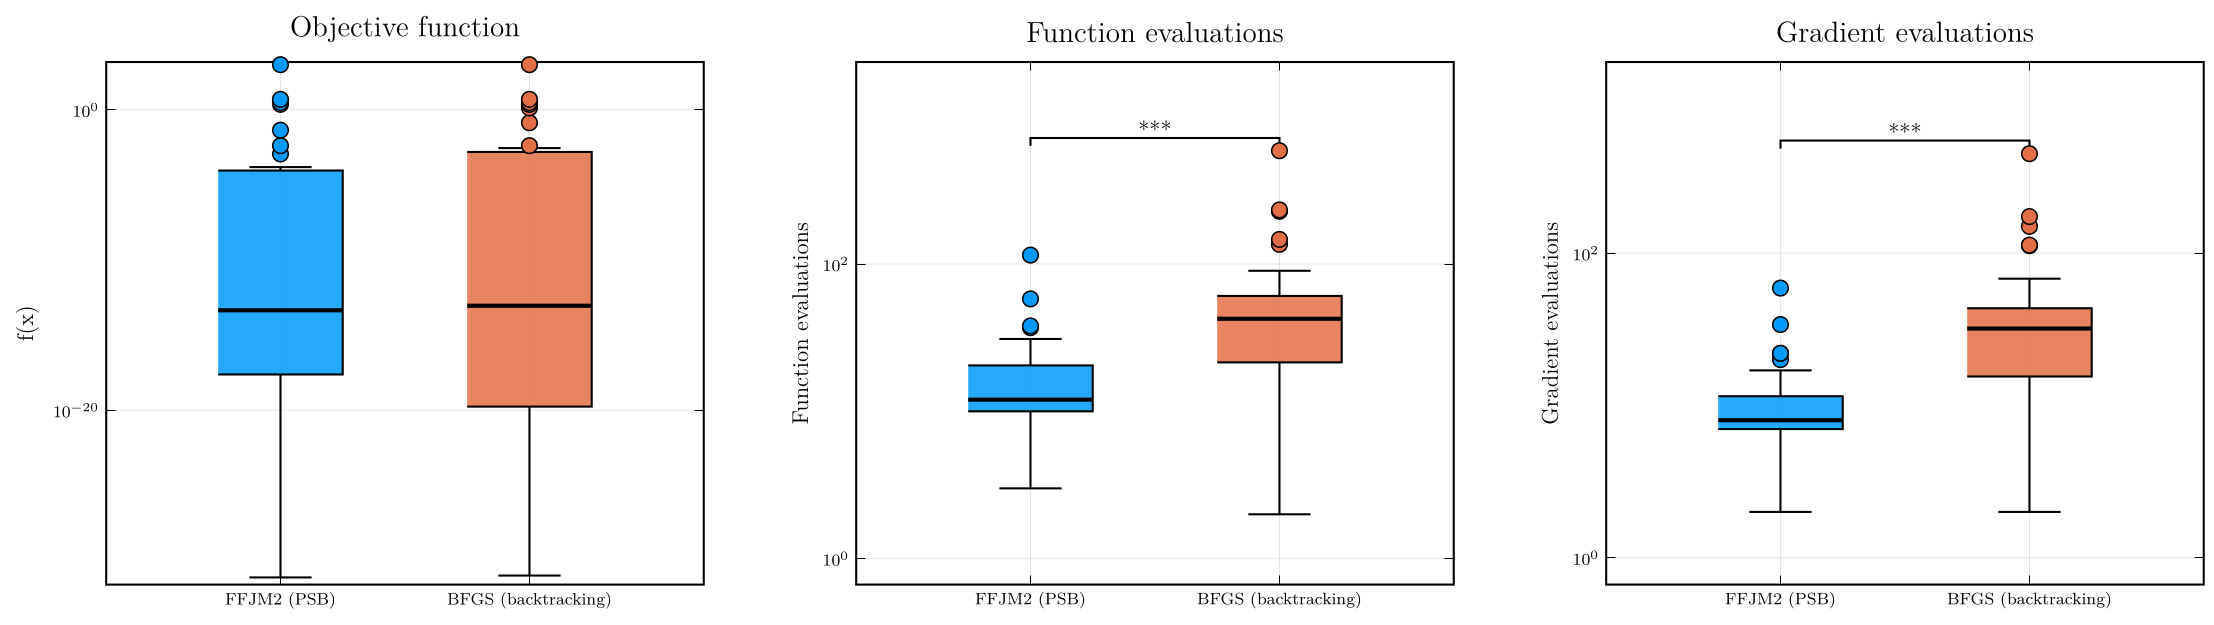
\includegraphics[width=\textwidth]{boxplot_ffjm2_bfgs.png}
    \caption{Comparison of FFJM2 (PSB) vs.\ BFGS (backtracking) on the MGH
        problems, restricted to runs where both methods converged by
        gradient norm. Final
        $f$ value, function evaluations, and gradient evaluations. Stars
        indicate significance under the Mann-Whitney U test
        \cite{MannWhitney1947} ($p < 0.05$:
        {*}; $p < 0.01$: {**}; $p < 0.001$: {***}).}
    \label{fig:boxplot-ffjm2-bfgs}
\end{figure}

As Figure~\ref{fig:boxplot-ffjm2-bfgs} shows, the objective function values
are not very different between the two methods: the p-value confirms
neither achieves a significantly better result. Function evaluations and
gradient evaluations, however, are different, and the p-value confirms
this difference is significant. FFJM2 therefore performs better than
BFGS in this respect, reaching a comparable solution at a much lower cost.

As an aside, the BFGS baseline above uses backtracking with quadratic
interpolation (order 2); Table~\ref{tab:bfgs-linesearches} checks how much
that particular choice of line search matters on its own, running
\texttt{Optim.BFGS} on the same 34 MGH problems with four line searches:
\texttt{LineSearches.HagerZhang()} (\texttt{Optim.jl}'s default), a
minimalist geometric backtracking with no interpolation (``order 1'',
always restarting from a fixed step of $1$), and \texttt{BackTracking}
with quadratic (order 2) and cubic (order 3) interpolation. ``Converged
(gradient)'' counts how many of the 34 problems stopped under the gradient
criterion; the remaining columns are mean~$\pm$~standard deviation over
all 34 problems (including the ones that stopped under a different
criterion).

\begin{table}[htbp]
\centering
\caption{Comparison of line searches for Optim.jl's BFGS on the 34 MGH problems.}
\label{tab:bfgs-linesearches}
\resizebox{\textwidth}{!}{%
\begin{tabular}{l r r r r r}
\toprule
Method & $f$ & Converged (gradient) & Iterations & Func.\ evals & Grad.\ evals \\
\midrule
Hager-Zhang & $1.29\times10^{3} \pm 7.36\times10^{3}$ & 33/34 & $66.91 \pm 120.92$ & $107.82 \pm 206.62$ & $107.82 \pm 206.62$ \\
Backtracking (order 1) & $2.49\times10^{7} \pm 1.45\times10^{8}$ & 30/34 & $51.56 \pm 93.74$ & $89.62 \pm 131.90$ & $52.47 \pm 93.75$ \\
Backtracking (order 2) & $1.29\times10^{3} \pm 7.36\times10^{3}$ & 32/34 & $61.59 \pm 99.26$ & $86.74 \pm 134.56$ & $62.56 \pm 99.17$ \\
Backtracking (order 3) & $1.29\times10^{3} \pm 7.36\times10^{3}$ & 31/34 & $56.91 \pm 89.47$ & $84.91 \pm 132.01$ & $57.85 \pm 89.33$ \\
\bottomrule
\end{tabular}%
}
\end{table}

\noindent
Hager-Zhang converges by gradient on the most problems (33/34) but at the
highest average cost, and its function/gradient evaluation counts always
match exactly --- it evaluates $f$ and $\nabla f$ together at every trial
point, unlike the three backtracking variants (which only need $\nabla f$
once a trial is accepted). Order-1 backtracking is the cheapest per
problem on average, but also the least reliable of the four (30/34).
Order-2 and order-3 sit in between on both counts. No single line search
dominates the other three on every metric; the differences are modest
next to the FFJM2 vs.\ BFGS gap of
Figure~\ref{fig:boxplot-ffjm2-bfgs}. The mean/std of $f$ is not a useful
per-problem quality measure here --- MGH problems span many orders of
magnitude at their true minima, so a couple of legitimately large-residual
problems (MGH16, $f\approx4.3\times10^4$; MGH06, $f\approx1.0\times10^3$)
already dominate the $1.29\times10^3\pm7.36\times10^3$ shared by
Hager-Zhang and orders 2--3, all three of which land on the same,
correct value on MGH10 ($f\approx44$) and everywhere else they converge.
Order-1 backtracking's much larger $2.49\times10^7\pm1.45\times10^8$ is a
genuine failure, not scale: it stalls at $x^0$ on MGH10 after a single
rejected trial ($f\approx8.5\times10^8$, seven orders of magnitude above
the correct value), the only case among the four where this happens.

A second aside: FFJM2's quartic subproblem (Section~2, Eq.~(18)/(21)) is
solved internally by Ipopt, but the paper's Algorithm 4.1 does not require
that particular choice. Table~\ref{tab:subproblem-solvers} checks how the
four solvers already available as \texttt{model\_solver} in \texttt{ffjm2}
--- Ipopt, BFGS (backtracking, same as above), BOBYQA, and MADS --- fare
when applied \emph{directly} to $0.5\|F(x)\|^2$ on the 34 MGH problems
(i.e., as if each one were, on its own, the whole optimizer, not just the
subproblem solver inside FFJM2's outer loop). Same columns as
Table~\ref{tab:bfgs-linesearches}; BOBYQA and MADS are derivative-free, so
their gradient-evaluation count is always $0$ and ``Converged (gradient)''
for them instead counts $\|\nabla f\|\le10^{-8}$ checked \emph{after} the
solver stops (Ipopt and BFGS report their own gradient-based termination
directly).

\begin{table}[htbp]
\centering
\caption{Comparison of the solvers available for FFJM2's internal
    subproblem, applied directly to $0.5\|F(x)\|^2$ on the 34 MGH problems.}
\label{tab:subproblem-solvers}
\resizebox{\textwidth}{!}{%
\begin{tabular}{l r r r r r}
\toprule
Method & $f$ & Converged (gradient) & Iterations & Func.\ evals & Grad.\ evals \\
\midrule
Ipopt & $1.88\times10^{5} \pm 1.09\times10^{6}$ & 32/34 & $69.53 \pm 103.06$ & $424.62 \pm 803.24$ & $71.53 \pm 103.06$ \\
BFGS (backtracking) & $1.29\times10^{3} \pm 7.36\times10^{3}$ & 32/34 & $61.59 \pm 99.26$ & $86.74 \pm 134.56$ & $62.56 \pm 99.17$ \\
BOBYQA & $1.47\times10^{10} \pm 8.56\times10^{10}$ & 10/34 & $572.71 \pm 699.05$ & $572.71 \pm 699.05$ & $0.00 \pm 0.00$ \\
MADS & $1.47\times10^{10} \pm 8.56\times10^{10}$ & 0/34 & $986.82 \pm 594.53$ & $986.82 \pm 594.53$ & $0.00 \pm 0.00$ \\
\bottomrule
\end{tabular}%
}
\end{table}

\noindent
Ipopt and BFGS are essentially tied on reliability (32/34) and land within
a factor of $2$ of each other on iterations and gradient evaluations, but
Ipopt needs about $5\times$ more function evaluations on average (it
solves a full barrier subproblem at each outer iteration). BOBYQA and MADS
are far behind on both counts: with no gradient to exploit, they need an
order of magnitude more evaluations and still only certify gradient
convergence on 10/34 (BOBYQA) or none at all (MADS) within the $2000$
function-evaluation budget. As Table~\ref{tab:ffjm2-subproblem-solvers}
below shows, this gap does \emph{not} carry over once these solvers are
used the way FFJM2 actually uses them --- as the resolver of the small,
cheap quartic model, rather than as the whole optimizer applied to the raw
residual. As in Table~\ref{tab:bfgs-linesearches}, the mean/std of $f$
is dominated by outliers rather than typical behavior, and here they point
to a genuine methodological limitation of the box these two derivative-free
solvers need (BOBYQA and MADS require finite bounds; both are given
$x^0\pm\mathrm{bound\_radius}$, $\mathrm{bound\_radius}=\max(10^3,
100\max(1,\|x^0\|))$): on MGH04, whose true minimizer is
$x^*\approx(10^6,\,2\times10^{-6})$, this box does not even contain
$x^*$ when $x^0=(1,1)$ gives $\mathrm{bound\_radius}=10^3$, so both solvers
stall at the box boundary ($f\approx5.0\times10^{11}$, versus
$\approx8\times10^{-28}$ for Ipopt/BFGS on the same problem) --- a box
sized from $\|x^0\|$ alone cannot help when $x^*$ is orders of magnitude
farther from $x^0$ than $x^0$ is from the origin. Ipopt's own outlier is
different in kind: on MGH10 it converges (\texttt{LOCALLY\_SOLVED}) to a
KKT point with $f\approx6.3\times10^6$, well above BFGS's
$f\approx44$ on the same problem, i.e.\ a genuine bad local
solution rather than a boundary artifact.

Table~\ref{tab:ffjm2-subproblem-solvers} repeats the comparison, but now
running \texttt{ffjm2} in full (\texttt{update=:psb}) on the same 34
problems, once per \texttt{model\_solver} --- i.e., Ipopt/BFGS/BOBYQA solve
only the small quartic model at each outer iteration, exactly as FFJM2
uses them, instead of standing in as the whole optimizer.
\texttt{function\_evaluations}/\texttt{gradient\_evaluations} here count
only calls to the real residual/Jacobian made by FFJM2's outer loop
(\texttt{residual(x)}/\texttt{jac(x)}); the internal solver's own work on
the quartic surrogate is tracked separately by \texttt{ffjm2} (fields
\texttt{model\_solves}/\texttt{model\_iterations}/
\texttt{model\_solve\_time\_seconds}, not shown) and never mixed into
these counts, so this is already an apples-to-apples measure of external
cost regardless of \texttt{model\_solver}. MADS is left out here: even at
a much smaller \texttt{model\_multistart} than the default ($10$ instead
of $1000$), a single easy problem (MGH01) took $\approx69$s in MADS alone
against $<0.1$s for BFGS/BOBYQA, making the default multistart impractical
across all 34 problems for this table.

\begin{table}[htbp]
\centering
\caption{FFJM2 (PSB), varying only \texttt{model\_solver}, on the 34 MGH problems.}
\label{tab:ffjm2-subproblem-solvers}
\resizebox{\textwidth}{!}{%
\begin{tabular}{l r r r r r}
\toprule
Method & $f$ & Converged (gradient) & Iterations & Func.\ evals & Grad.\ evals \\
\midrule
FFJM2 (PSB, Ipopt) & $1.29\times10^{3} \pm 7.36\times10^{3}$ & 31/34 & $15.12 \pm 21.90$ & $30.21 \pm 49.59$ & $16.12 \pm 21.90$ \\
FFJM2 (PSB, BFGS) & $1.29\times10^{3} \pm 7.36\times10^{3}$ & 31/34 & $15.26 \pm 21.99$ & $30.26 \pm 48.63$ & $16.26 \pm 21.99$ \\
FFJM2 (PSB, BOBYQA) & $1.29\times10^{3} \pm 7.36\times10^{3}$ & 30/34 & $39.74 \pm 108.86$ & $57.68 \pm 127.48$ & $40.74 \pm 108.86$ \\
\bottomrule
\end{tabular}%
}
\end{table}

\noindent
The gap seen in Table~\ref{tab:subproblem-solvers} almost disappears here:
Ipopt and BFGS as \texttt{model\_solver} are essentially indistinguishable
(31/34, within $1\%$ of each other on every column), and even BOBYQA ---
which needed an order of magnitude more evaluations and converged on only
10/34 when applied directly to the raw residual --- falls behind by only
one problem (30/34) and roughly $2.6\times$ more outer iterations on
average, not $10\times$. All three land on the same $f$ statistics, again
driven by the legitimately large-residual MGH16/MGH06 rather than any
failure. This is exactly the effect anticipated when this experiment was
designed (\texttt{teste.jl}): FFJM2's own outer loop --- the ratio test
that rejects a bad step and grows $\mu$, and the full Hessian reset that
follows a bad ratio (see the discussion of $\mu$ in the Introduction)
--- compensates for a mediocre subproblem solution, so a weaker
\texttt{model\_solver} costs a few extra outer iterations rather than
failing outright. FFJM2 still defaults to Ipopt --- tied with BFGS on
reliability (31/34) and within a step or two of it on every problem where
they differ (worst case MGH10, $121$ outer iterations against BFGS's
$120$) --- but the choice matters far less than
Table~\ref{tab:subproblem-solvers} alone would suggest.





\section{Coeficient estimation problem}

The Saint-Venant equations \cite{castro,leveque,porto,saintvenant} 
  describe the flow of fluids in natural channels. The state variables that describe a natural channel vary
  with respect to $x \in [x_{min}, x_{max}]$ (position, usually measured  in meters) and $t \in [t_{min},t_{max}]$ (time, usually
  measured in seconds).
  We define:

\begin{itemize}
\item $z(x, t)$: surface elevation
\item $h(x,t) = z(x,t) - z_b(x)$: river depth at $(x,t)$
\item $A(x,t)$: cross-sectional wetted area
\item $Q(x,t)$: flow rate
\item $P(x,t)$: wetted perimeter
\item $R(x,t) = A(x,t) / P(x,t)$: hydraulic radius
\item $g$: acceleration of gravity (approximately $9.81 m/s^2$)
\end{itemize}

 The Saint-Venant equations consist of two main components:
Equation~(\ref{massa})
describes mass conservation and equation~(\ref{momentong}) represents
conservation of the linear momentum.                                


\begin{equation} \label{massa}
\frac{\partial A}{\partial t} + \frac{\partial Q}{\partial x} = 0
\end{equation}
and
\begin{equation} \label{momentong}
\frac{\partial Q}{\partial t} + \frac{\partial}{\partial x}
\left(\frac{Q^2}{A}\right) + g A \frac{\partial z}{\partial x} +
\frac{n_g^2 Q|Q|}{A R^{4/3}} = 0.
\end{equation} 

 The Manning (also called Yen-Manning \cite{bcgmr}) coefficient $n_g$ represents roughness \cite{bcgmr}.
Typically, given the inlet discharge $Q(x_{min}, t)$ for $t \in [t_{min}, t_{max}]$, initial conditions $A(x, t_{min})$ 
and $Q(x, t_{min})$, and the coefficient $n_g$, numerical methods compute the values of $Q(x, t)$ and $A(x, t)$ at a set
 of discrete ``grid points" $(x_\nu, t_\nu)$. Unfortunately, the Yen-Manning coefficient  $n_g$ is often unknown for natural channels
 and can vary with position $x$ and even time $t$. {For more details, see \cite{bcgmr}}.  

 This research assumes that the  Manning coefficient $n_g$ varies with position $x$, and that a set of elevation
 observations $z_{obs}(x_\nu, t_\nu)$ are available at $n_{obs}$ distinct locations and times, indexed by $\nu = 1, \ldots, n_{obs}$. 
Consequently, the spatial distribution of $n_g(x)$, discretized over a suitable grid, becomes an unknown component of our problem.
 Furthermore, to ensure physically plausible results, minimal variation will be required for a function $n_g(x)$ that minimizes
 spatial oscillations while fitting the solution of the Saint-Venant equations to the observations.

 Based on this, is possiblem consider we have a function genereted by the PDE solution $Z(\eta) = 
 [z_1(x_1, t_1, \eta), z_2(x_2, t_2, \eta), \ldots, z_{n_{obs}}(x_\nu, t_\nu, \eta)]^T$,
 $\overline{z} = [z_{obs}(x_1, t_1), z_{obs}(x_2, t_2u), \ldots, z_{obs}(x_{n_{obs}}, t_{n_{obs}})]^T$ we want to find $\eta$ 
 as solving a sistem of problems given for $F(\eta) = Z(\eta) - z = 0$.
























\begin{thebibliography}{9}

\bibitem{DennisWolkowicz1993}
J. E. Dennis, Jr. and H. Wolkowicz, \emph{Sizing and least-change secant
methods}, SIAM J. Numer. Anal., 30 (1993), pp.~1291--1314.

\bibitem{LuksanSpedicato2000}
L. Luk\v{s}an and E. Spedicato, \emph{Variable metric methods for
unconstrained optimization and nonlinear least squares}, J. Comput. Appl.
Math., 124 (2000), pp.~61--95.

\bibitem{MannWhitney1947}
H. B. Mann and D. R. Whitney, \emph{On a test of whether one of two random
variables is stochastically larger than the other}, Ann. Math. Statist.,
18 (1947), pp.~50--60.

\bibitem{Mogensen2018}
P. K. Mogensen and A. N. Riseth, \emph{Optim: A mathematical optimization
package for Julia}, J. Open Source Software, 3 (2018), p.~615.

\bibitem{MoreGarbowHillstrom1981}
J. J. Mor\'e, B. S. Garbow, and K. E. Hillstrom, \emph{Testing
unconstrained optimization software}, ACM Trans. Math. Software, 7 (1981),
pp.~17--41.

\bibitem{Powell1970}
M. J. D. Powell, \emph{A new algorithm for unconstrained optimization}, in
Nonlinear Programming, J. B. Rosen, O. L. Mangasarian, and K. Ritter, eds.,
Academic Press, New York, 1970, pp.~31--65.

\end{thebibliography}





\end{document}
